% !TeX spellcheck = en_US
\documentclass{beamer}
\usepackage{caption}
\usepackage{subcaption}
\usepackage[autostyle]{csquotes}  
%\usepackage[
%backend=biber,
%style=authoryear,
%citestyle=authoryear 
%]{biblatex}
%
%\addbibresource{../literature/bibliography.bib}

\usetheme{rwth}
\MakeOuterQuote{"}
%\title{Conformance Checking Using Embeddings and its Applicability in the Internet of Things}
%\author{Jan Kruska}
%\date{\today}

\newcommand{\figures}{../figures/}

\newcommand{\pro}{\item[\color{green}\textbf{+}\color{black}]}
\newcommand{\con}{\item[\color{red}\boldmath{$-$}\color{black}]}
\newcommand{\green}[1]{\color{green}\textbf{#1}\color{black}}

\logo{
\includegraphics{figures/rwth_pads_en_rgb}}

% Adjust your information
\title{Conformance Checking Using Embeddings and its Applicability in the Internet of Things}
%\subtitle{Bachelor/Master Thesis OR Seminar Paper for Seminar ``XY''}
\date{\today}
\newcommand{\firstname}{Jan}
\newcommand{\lastname}{Kruska}
\newcommand{\matrNo}{414967}
\newcommand{\email}{jan.kruska@rwth-aachen.de}
\newcommand{\studyProgram}{\ifdefined\BACHELOR{} Bachelor \else Master \fi Computer Science}

% Adjust first supervisor information
\newcommand{\firstsupervisor}{first supervisor}
\newcommand{\firstsupervisorchair}{chair of first supervisor}
\newcommand{\firstsupervisoruniversity}{RWTH Aachen University}

% Adjust second supervisor information
\newcommand{\secondsupervisor}{second supervisor}
\newcommand{\secondsupervisorchair}{chair of second supervisor}
\newcommand{\secondsupervisoruniversity}{RWTH Aachen University}


% Adjust advisor information
\newcommand{\firstadvisor}{first advisor}
\newcommand{\firstadvisorchair}{chair of first advisor}
\newcommand{\firstadvisoruniversity}{RWTH Aachen University}

% comment these lines out if you have only one advisor
\newcommand{\secondadvisor}{second advisor}
\newcommand{\secondadvisorchair}{chair of second advisor}
\newcommand{\secondadvisoruniversity}{RWTH Aachen University}
\author[\firstname]{\firstname~\lastname~\email}
\institute[RWTH]{RWTH Aachen University}

\begin{document}
	\beamertemplatenavigationsymbolsempty
	\addtobeamertemplate{navigation symbols}{}{%
		\usebeamerfont{footline}%
		\usebeamercolor[fg]{footline}%
		\hspace{1em}%
		\insertframenumber
	}
% Title page with a 1/3rd size picture
\setbeamercolor{title page bar}{fg=white}
\setbeamertemplate{title page}[rwth][figures/title_small]{}
\setbeamertemplate{bibliography item}{\insertbiblabel}
\begin{frame}[plain]
	\vspace{1cm}
	\titlepage
	
	\vspace{-6em}
	\parbox{0cm}{
		\begin{tabbing}
			\=\textbf{\firstname~\lastname}\=\\[0.4em]
			\=Study Program: \studyProgram~~~\=Matr.-Nr.:\matrNo\\[0.4em]
			\=Chair of Process and Data Science \=\\%[0.4em]
			\={Seminar:}~~~\=Business Processes and the Internet of Things\\
%			\>                 \>\secondsupervisor\\[0.4em]
%			\={Advisor}:       \>\firstadvisor\ifdefined\secondadvisor\\
%			\>                 \>\secondadvisor\\[0.4em]
%			\fi
		\end{tabbing}
	}
\end{frame}
	\begin{frame}
		\frametitle{Table of Contents}
		\tableofcontents
	\end{frame}
	\section{Motivation}
	\begin{frame}
		\frametitle{Motivation}
		%\begin{center}	
		%\end{center}
		\begin{itemize}
			\item Traditional approaches (replay and alignments) are able to measure conformance, but have meaningful disadvantages:
			\begin{itemize}
				\item replay based approaches suffer form inaccurate diagnostics through phenomena like token flooding
				\item alignments suffer from high computational complexity
			\end{itemize}
			\item[$\Rightarrow$] There is interest in finding alternatives to traditional approaches
			\item<2-> Conceptually, Natural Language Processing and Business Process management share some important characteristics. Both deal with sequences (sentences/traces) of words/activities and aim to define similarity measures between those.
		\end{itemize}
		\begin{block}<2->{Research Question:}
			Are adaptations of NLP techniques feasible solutions for problems in the BPM field, specifically for the problem of conformance checking?
		\end{block}
		\temporal<3->{}{\alert{Theoretical exploration in previous paper \cite{KBWe18}, here \cite{PBWe20} implementation and evaluation was the main concern}}{}
	\end{frame}

\begin{frame}
	\frametitle{Embeddings Introduced in \cite{KBWe18}}
	\begin{itemize}
		\item<-3> \emph{act2vec}:  \temporal<2->{Analogous to \emph{word2vec} (Does not use activity attributes currently)}{\green{Base building block, simple, robust}}{}
		\item<-3> \emph{trace2vec}:  \temporal<2->{Utilizes \emph{act2vec} and adds a paragraph vector, analogous to \emph{doc2vec}}{\green{Useful for direct trace comparison}}{}
		\item<-2> \emph{log2vec}:  \temporal<2->{Extends \emph{trace2vec} by including an averaging operation, to create an embedding for the whole log}{\alert{Too coarse}}{}
		\item<-2> \emph{model2vec}:  \temporal<2->{Embedding of the graph structure of a model by performing random walks}{\alert{Complex, not very robust, not useful for log/model comparisons}}{}
	\end{itemize}
\end{frame}

	\section{Structure of Embedding based Conformance Checking}
	\begin{frame}
		\frametitle{Conformance Checking using Activity and Trace Embeddings}
		\begin{columns}
			\column{0.5\textwidth}
			\begin{enumerate}
				\item Given a model play it out to obtain a so called model log
				\item Train activity embeddings (\emph{act2vec}) based on real and model logs
				%\item Any trace is a sequence of activities. Given an embedding (dis)similarity metrics can be defined
				\item Using a (dis)similarity metric pairwise compare all traces in real and model log.
			\end{enumerate}
			\begin{block}{Definition of Fitness and Precision}
				Then the best similarity between a real trace and all model traces is a measure for fitness. Conversely, the best similarity between a model trace and all real traces is a measure for precision.
			\end{block}
		\column{0.4\textwidth}
		\begin{figure}
			\includegraphics[width=1\linewidth, height=0.6\paperheight, keepaspectratio]{\figures structure}
			\caption{The General Structure of the Approach}
			\label{fig:structure}
		\end{figure}
	\end{columns}
	\end{frame}
	
	
	\begin{frame}
		\frametitle{Used Dissimilarity Functions}
\begin{columns}[t]
	\column{.7\textwidth}
		\begin{enumerate}
			\item \textbf{Word Mover's distance} \cite{KSKW15} How much "work" is needed to transform one distribution of dirt on piles into another. Both distance between piles and amount of dirt on piles matter.
			\item \textbf{Iterative Constraint Transfers} \cite{AtMi18} WMD has cubic complexity in the dictionary size, which makes it unattractive. ICT is a linear time approximation of WMD obtained by relaxing one of the constraints of the LP.
			\item \textbf{\emph{trace2vec}} \cite{KBWe18} Analogously to \emph{doc2vec}, train an embedding of bags of activities called \emph{trace2vec}. Use cosine similarity to directly compare traces in the trace embedding space.
		\end{enumerate}
	\alert{The obtained metrics are not proper fitness metrics, i.e. they do not fall within the interval $[0,1]$. As such, quantitative analyses are not really possible at this point.}
		\column{.3\textwidth}
	\begin{figure}
		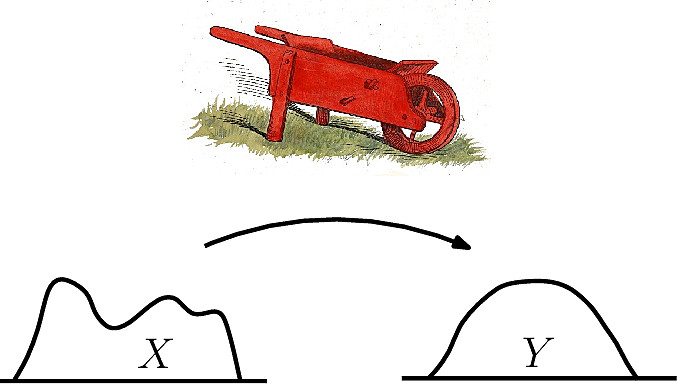
\includegraphics[width=1\linewidth, keepaspectratio]{figures/emd}
	\end{figure}
\end{columns}
	\end{frame}
	
	\section{Experiments}
	\begin{frame}
		\frametitle{Experimental Setup}
		In the paper three experiments were performed:
		\begin{enumerate}
			\item Noise: Applying noise to a varying amount of traces/ varying amount of noise applied to same amount of traces. Investigate how the methods react. Do they deteriorate smoothly?
			\item Discovery: Discover model using different miners, determine fitness and precision using the three proposed methods as well as alignment fitness and precision \cite{Aals16}, behavioural fitness \cite{GMVB09} and ETC precision \cite{MuCa10}.
			\item Scaling: Vary log and dictionary sizes (number of activities). Compare runtimes \alert{No runtimes of traditional methods were included.}
		\end{enumerate}

	\end{frame}
\begin{frame}
	\frametitle{How to get the Logs?}
	\begin{figure}
		\includegraphics[width=1\textwidth]{\figures process-tree}
		\caption{A process tree generated by pm4py using parameters: Min 15, Mode 30, Max 45, sequence 0.75, parallel 0.25. }
		\label{fig:process-tree}
	\end{figure}
\end{frame}
	\begin{frame}
		\frametitle{Random Trees}
		Random trees were generated using pm4py and the following configurations:
		
		\begin{center}
		\begin{tabular}{lll}
			Min & Mode & Max \\
			5 & 10 & 15 \\
			10 & 20 & 30 \\
			15 & 30 & 45 \\
		\end{tabular}
	\hspace{40pt}
		\begin{tabular}{llll}
			Sequence & Parallel & Choice & Loop \\
			0.75 & 0.25 & 0 & 0 \\
			0.75 & 0 & 0.25 & 0 \\
			0.5 & 0.25 & 0.25 & 0 \\
			0.25 & 0.25 & 0.25 & 0.25 \\
		\end{tabular}
	\end{center}

		Using these parameters $3\times4=12$ trees were generated.
		Then from each of those the "real" logs of 1000 traces were gathered by play-out.
		
		The scaling experiment used different unspecified trees varying the amount of activities and the size of the played-out log.
	\end{frame}
	
	
	\begin{frame}
		\frametitle{Noise Experiment}
		The goal of the noise experiments was to investigate whether the methods are well-behaved and conform to the expectations.
		\begin{figure}
			\centering
			\begin{subfigure}[b]{0.45\textwidth}
				\centering
				\includegraphics[width=\textwidth]{\figures noise-first}
				\caption{Average of first noise experiment (Varying trace percentage).}
				\label{fig:noise-first}
			\end{subfigure}
			\hfill
			\begin{subfigure}[b]{0.45\textwidth}
				\centering
				\includegraphics[width=\textwidth]{\figures noise-second}
				\caption{Average of second noise experiment (Varying amount of noise applied to trace).}
				\label{fig:noise-second}
			\end{subfigure}
		\end{figure}
	\end{frame}
	
	
	\begin{frame}
		\frametitle{Discovery Experiment}
		In the Discovery experiment the embedding-based methods are evaluated against reference methods using different trees and discovery algorithms.
		\begin{figure}
			\centering
			\begin{subfigure}[b]{0.49\textwidth}
				\centering
				\includegraphics[width=\textwidth]{\figures fitness}
				\caption{Fitness}
				\label{fig:fitness}
			\end{subfigure}
			\hfill
			\begin{subfigure}[b]{0.49\textwidth}
				\centering
				\includegraphics[width=\textwidth]{\figures precision}
				\caption{Precision}
				\label{fig:precision}
			\end{subfigure}
			\caption{Fitness and Precision for different tree, discovery technique pairings for the three proposed techniques as well as the two verification techniques.}
			\label{fig:discovery}
		\end{figure}
	\end{frame}
	
	\begin{frame}
		\frametitle{Results from Noise \& Discovery Experiments}
		\begin{itemize}
			\item Overall, noise behaves as expected
			\item Again, quantitative analyses can not be made from this data!
			\item Very often, the NLP and reference methods agree on perfect fitness or precision
			\item For imperfect values, the methods also seem to move in a similar direction, though further research is needed.
			\item Validation techniques should not be seen as normative, since both of these also significantly disagree for some models. 
		\end{itemize}
	\end{frame}
	
	
	\begin{frame}
		\frametitle{Scaling Experiment}
		The goal of the scaling experiment was to determine how the methods scale regarding vocabulary and log size
		\begin{figure}
			\includegraphics[width=1\linewidth, height=0.55\paperheight, keepaspectratio]{\figures scaling}
			\caption{Runtimes for all three methods for varying sizes of logs and dictionaries.}
			\label{fig:scalability}
		\end{figure}
	\end{frame}
	
	
	\begin{frame}
		\frametitle{Results from Scaling Experiment}
		\begin{itemize}
			\item Note that WMD was calculated using a library with NumPy efficiency, whereas ICT was implemented in pure python. Yet unoptimized ICT already rivals WMD, very likely an attractive alternative.
			\item ICT scales well, \emph{trace2vec} stays the same with dictionary size
			\item All methods scale roughly quadratically with log-size, since the number of necessary comparisons grows quadratically
			\item log-comparison method. Performance dependent on model complexity. How many traces are needed to describe the model sufficiently well.
		\end{itemize}
	\end{frame}
	
	\begin{frame}
		\frametitle{Scientific Replicability of Experiment Results}
		\begin{block}<1->{Source Code}
				 Code\footnote{https://github.com/jaripeeperkorn/Conformance-checking-using-activity-and-trace-embeddings} for both experiments and implementation is available. As such, it seemed useful to evaluate how well the results are reproducible using that code.
		\end{block}
		\begin{itemize}
%			 \pro<1-> Code for experiments  is available and well-organized
			 \pro<2-> Implementation and experiments are separated, should allow for relatively easy reuse of their embedding solution
			 \con<3-> Experiment scripts only run experiment for one configuration. Reproducing their results requires manually entering all parameter combinations used (e.g. log and vocabulary size for the scalability experiment) and noting down results.
			 \con<4-> Output format
			 \begin{itemize}
			 	\item<4-> Results outputted as plain text in Jupyter Notebook, that needs to be manually copied
			 	\item<4-> This makes further processing of results tedious and more error prone
			 	\item<4-> Suggestion: Instead collect results in dataframe and save as csv
			 \end{itemize}
			 \con<5-> No code included to create the figures displayed in the paper.
			 \con<6-> Alignment fitness and precision, Behavioral fitness and ECT precision are not calculated in the discovery experiment script.
			 \item<7->\color{red}Another performance experiment comparing these embedding-based methods to the reference methods would be desirable. Since Alignment, Behavioral fitness and ECT calculations were not present in the discovery script, this was not possible to do in a reasonable time frame for the seminar.\color{black}
		\end{itemize}
	\begin{alertblock}<7->{block title}<action specification>
		Another performance experiment comparing these embedding-based methods to the reference methods would be desirable. Since Alignment, Behavioral fitness and ECT calculations were not present in the discovery script, this was not possible to do in a reasonable time frame for the seminar.
	\end{alertblock}
%	\temporal<7->{}{\alert{Another performance experiment comparing these embedding-based methods to the reference methods would be desirable. Since Alignment, Behavioral fitness and ECT calculations were not present in the discovery script, this was not possible to do in a reasonable time frame for the seminar.}}{}
	\end{frame}
	
	\section{Application in the Internet of Things}
	\begin{frame}
		\frametitle{Internet of Things}
		\begin{block}<1->{Performance and Scaling}
			\begin{itemize}
				\item Good scaling w.r.t number of activities could be necessary in scenarios with real time requirements and large amounts of data.
				\item Learned embeddings could be shared between devices, moving work out of the evaluation to a preceding training step.
			\end{itemize}
		\end{block}
	
	\begin{block}<2->{Online Process Mining}
		\begin{itemize}
			\item Streaming capabilities are a bigger priority in an IoT context. Difficult to do without explicit end-of-trace knowledge, at least prefix-conformance approach from \cite{ZBK*19} should be easily replicable. Whether embeddings could lead to better approaches constitutes a whole work in itself.
			\item More automated, embeddings could be retrained/improved regularly based on new observed data.  
		\end{itemize}
	\end{block}

\begin{block}<3->{Utilization of more complex NLP techniques}
	\begin{itemize}
		\item Possibly much more complex tasks. E.g. an analogy to predictive text, i.e. predicting the next event given a sequence of observed events.
	\end{itemize}
\end{block}
	\end{frame}

\section{Conclusion and Outlook}
\begin{frame}
	\frametitle{Embeddings for BPM}
	\begin{exampleblock}{Do not lose sight of the more general benefits!}
		While this paper dealt mostly with embeddings for conformance checking the possibilities when moving from generic objects (traces) to vector space embeddings should not be understated and are emphatically not limited to conformance checking. 
	\end{exampleblock}
	
	
	\begin{itemize}
		\item Other methods essentially utilize binary activity equality and relatively simple models for trace comparison. Embeddings provide much more fine grained relationships between embedded objects.
		\item This opens up a plethora of techniques that reach far beyond conformance checking.
		\item Especially automatic clustering of similar activities, as is achieved by an embedding could be potentially very useful.
	\end{itemize}
	 
\end{frame}

\begin{frame}
	\frametitle{Conclusion \& Future Work}
	\begin{itemize}
		\item In general very interesting initial results were obtained that warrant further research
		\item The performed experiment are not sufficient to reliably ascertain how well embedding-based methods perform in real world scenarios. Experiments with real logs should follow.
		\item The metrics used at the moment are not proper fitness/precision metrics (Not in $[0,1]$).
		\item WMD and ICT do not take activity order into account, \emph{trace2vec} only does so during training
		\item Given the work it also seems feasible to move on to more complicated NLP techniques:
		\begin{itemize}
			\item $n$-grams
			\item Embeddings from Language Models
			\item Global Vectors for Word Representation
			\item Recurrent Neural Networks
		\end{itemize}
	\end{itemize}
\end{frame}

\section*{References}
\begin{frame}[allowframebreaks]
%	\frametitle{References}
	\bibliographystyle{apalike}
%	\bibliographystyle{authoryear}
	\bibliography{../literature/bibliography}
%	\printbibliography
\end{frame}

\begin{frame}{}
	\centering \Huge
	\emph{Thank you for your attention!}
	
	\emph{Questions?}
\end{frame}
	
\end{document}